\chapter{Folding and Tracing Constructions}
\begin{quote} 
We don't even know if Foldspace introduces us to one universe or
many\dots

\hfill---Frank Herbert
\end{quote}

\section{Constructions}

While origami as an art form is quite ancient, folding and tracing constructions
in mathematics are relatively new. The earliest mathematical
discussion of folding and tracing constructions that I know of appears in
T.\ Sundara Row's book \textit{Geometric Exercises in Paper Folding}
\cite{row}, first published near the end of the Nineteenth Century. In
the Twentieth Century it was shown that every construction that is
possible with a compass and straightedge can be done with
folding and tracing. Moreover, there are constructions that are possible via
folding and tracing that are \textit{impossible} with compass and straightedge
alone. This may seem strange as you can draw a circle with a compass,
yet this seems impossible to do via paper-folding. We will address
this issue in due time. Let's get down to business---here are the
rules of folding and tracing constructions:


\subsubsection*{Rules for Folding and Tracing Constructions}
\begin{enumerate}
\item You may only use folds, a marker, and semi-transparent paper.
\item Points can only be placed in two ways:
\begin{enumerate}
\item As the intersection of two lines. 
\item By marking ``through'' paper onto a previously placed
  point. Think of this as when the ink from a permanent marker
  ``bleeds'' through the paper.
\end{enumerate}
\item Lines can only be obtained in three ways:
\begin{enumerate}
\item By joining two points---either with a drawn line or a fold.
\item As a crease created by a fold. 
\item By marking ``through'' paper onto a previously placed
  line.
\end{enumerate}
\item One can only fold the paper when:
\begin{enumerate}
\item Matching up points with points.
\item Matching up a line with a line.
\item Matching up two points with two intersecting lines.
\end{enumerate}
\end{enumerate}


Now we are going to present several basic constructions. We will
proceed by the order of difficulty of the construction.


\begin{con}[Transferring a Segment]\index{folding and tracing!transferring a segment}  
Given a segment, we wish to move it so that it starts on a given
point, on a given line.
\end{con}


\begin{con}[Copying an Angle]\index{folding and tracing!copying an angle} 
Given a point on a line and some angle, we wish to copy the given
angle so that the new angle has the point as its vertex and the line
as one of its edges.
\end{con}

Transferring segments and copying angles using folding and tracing without a
``bleeding marker'' can be tedious. Here is an easy way to do it: 
\begin{center}
\textbf{Use 2 sheets of paper and a pen that will mark through multiple
sheets.}
\end{center}

\begin{ques} 
Can you find a way to do the above constructions without using a
marker whose ink will pass through paper?
\end{ques}
\QM

\begin{con}[Bisecting a Segment]\index{folding and tracing!bisecting a segment} 
Given a segment, we wish to cut it in half.
\begin{enumerate}
\item Fold the paper so that the endpoints of the segment meet.
\item The crease will bisect the given segment.
\end{enumerate}
\[
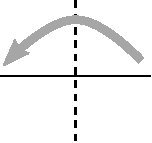
\includegraphics{../graphics/origamiBisect.pdf}
\]
\end{con}

\begin{ques} 
Which rule for folding and tracing constructions are we using above?
\end{ques}
\QM


\begin{con}[Perpendicular through a Point]\index{folding and tracing!perpendicular through a point}  
Given a point and a line, we wish to construct a line perpendicular to
the original line that passes through the given point.
\begin{enumerate}
\item Fold the given line onto itself so that the crease passes though
  the given point.
\item The crease will be the perpendicular line.
\end{enumerate}
\[
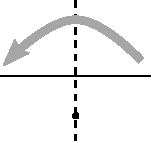
\includegraphics{../graphics/origamiPerpPoint.pdf}
\]
\end{con}

\begin{ques} Which rule for folding and tracing constructions are we using above?
\end{ques}
\QM




\begin{con}[Bisecting an Angle]\index{folding and tracing!bisecting an angle} 
We wish to divide an angle in half.
\begin{enumerate}
\item Fold one leg of the angle to the other leg so that
  the crease passes though the vertex of the angle.
\item The crease will bisect the angle.
\end{enumerate}
\[
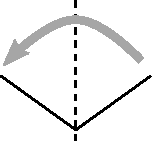
\includegraphics{../graphics/origamiBangle.pdf}
\]
\end{con}


\begin{ques} Which rule for folding and tracing constructions are we using above?
\end{ques}
\QM



\begin{con}[Parallel through a Point]\index{folding and tracing!parallel through a point} 
 Given a line and a point not on the line, we wish to construct another line parallel
 to the first that passes through the given point.
\begin{enumerate}
\item Fold a perpendicular line through the given point.
\item Fold a line perpendicular to this new line through the given
  point.
\end{enumerate}
\[
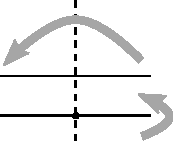
\includegraphics{../graphics/origamiParaPoint.pdf}
\]
\end{con}



Now there may be a pressing question in your head:

\begin{ques} 
How the heck are we going to fold a circle?
\end{ques}

First of all, remember the definition of a circle:

\begin{dfn}\index{circle}
A \textbf{circle} is the set of points that are a fixed distance from
a given point.
\end{dfn}

\begin{ques} Is the center of a circle part of the circle?
\end{ques}
\QM

Secondly, remember that when doing compass and straightedge
constructions we can \textbf{only} mark points that are intersections
of lines and lines, lines and circles, and circles and circles. Thus
while we technically draw circles, we can only actually mark certain
points on circles.  When it comes to folding and tracing constructions, drawing a
circle amounts to marking points a given distance away from a given
point---that is exactly what we can do with compass and straightedge
constructions.


\begin{con}[Intersection of a Line and a Circle]
\index{folding and tracing!intersection of a line and a circle} We wish to
construct the points where a given line meets a given circle. Note: A
circle is given by a point on the circle and the center point.
\begin{enumerate} 
\item Fold the point on the circle onto the given line so that the
  crease passes through the center of the circle.
\item Mark this point though both sheets of paper onto the line.
\end{enumerate}
\[
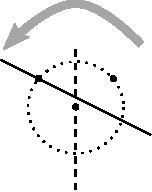
\includegraphics{../graphics/origamiCircLine.pdf}
\]
\end{con}

\begin{ques} Which rule for folding and tracing constructions are we using above?
\end{ques}
\QM

\begin{ques} How could you check that your folding and tracing construction is correct?
\end{ques}
\QM

\begin{con}[Equilateral Triangle]\index{folding and tracing!equilateral triangle} 
We wish to construct an equilateral triangle given a segment which is one of the sides.  (We say we are ``given the length of one side''.)
\begin{enumerate} 
\item Bisect the segment.
\item Fold one end of the segment onto the bisector so that the crease
  passes through the other end of the segment. Mark this point onto
  the bisector.
\item Connect the points.
\end{enumerate}
\[
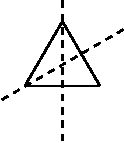
\includegraphics{../graphics/origamiTriangle.pdf}
\]
\end{con}

\begin{ques} Which rules for folding and tracing constructions are we using above?
\end{ques}
\QM







\begin{con}[Intersection of Two Circles]\index{folding and tracing!intersection of two circles} 
We wish to find the intersection of two circles, each given by a center point and a
point on the circle. 
\begin{enumerate}
\item Use four sheets of tracing paper. On the first sheet, mark the
  centers of both circles. On the next two sheets, mark the center and
  point on each of the circle---one circle per sheet. 
\item Simply move the two sheets with the centers and points on the
  circles, so that the centers are over the centers from the first
  sheet, and the points on the circles coincide. Now on the fourth
  sheet, mark all points.
\end{enumerate}
\end{con}

\begin{ques}
How do you use folding and tracing to construct a regular hexagon?
What other regular polygons can you construct?
\end{ques}
\QM


%% Think about the definition of a circle. In a similar fashion we can
%% define other common geometric figures:


%% \begin{dfn} 
%% Given a point and a line, a \textbf{parabola}\index{parabola} is the
%% set of points such that each of these points is the same distance from
%% the given point as it is from the given line.
%% \[
%% 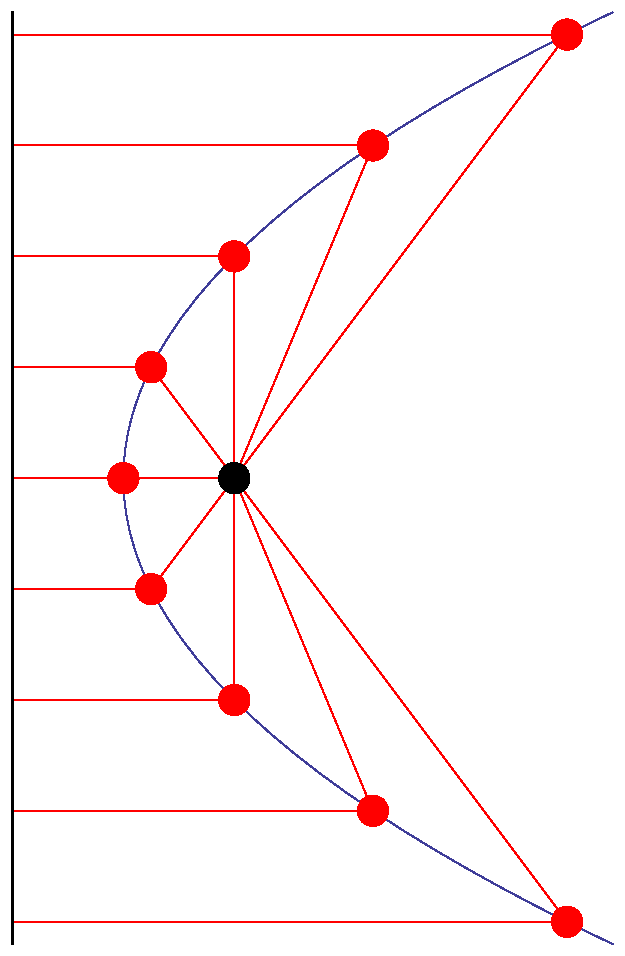
\includegraphics[angle=90,scale=.4]{../graphics/parabolapointline.pdf}
%% \]
%% \end{dfn}

%% We can also form a parabola from an \textit{envelope of
%%   tangents}:\index{envelope of tangents}
%% \[
%% 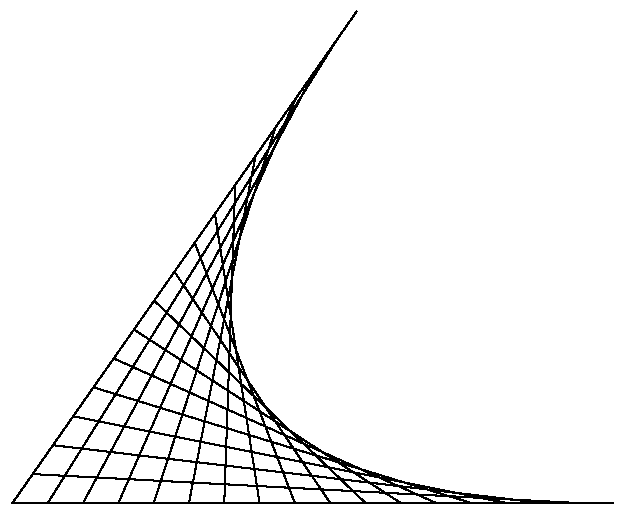
\includegraphics[scale=.6]{../graphics/envelope.pdf}
%% \]
%% Using a similar idea we can essentially obtain a parabola using
%% folding and tracing.

%% \begin{con}[Parabola]\index{folding and tracing!parabola} 
%% Given a point and a line we wish to construct a parabola.
%% \begin{enumerate}
%% \item Make a series of equally spaced marks on your line. 
%% \item Fold the point onto the marks.
%% \item Repeat the above step until an envelope of tangents forms.
%% \end{enumerate}
%% \end{con}

%% \begin{ques} 
%% Considering the definition of the parabola, can you explain why the
%% above construction makes sense?
%% \end{ques}
%% \QM

%% \begin{ques} Can you give a compass and straightedge construction of a parabola?
%% \end{ques}
%% \QM

%% Our final basic folding and tracing construction is one that \textbf{cannot} be
%% done with compass and straightedge alone.



%% \begin{con}[Angle Trisection\footnote{This construction was discovered by S.T.\ Gormsen and verified by S.H.\ Kung.}]\index{trisecting the angle}\index{folding and tracing!trisecting the angle}
%% We wish to divide an angle into thirds.
%% \begin{enumerate}
%% \item Bisect the given angle.
%% \item Find two points (one on each leg of the angle) equidistant from the vertex of the angle.
%% \item Fold the two points found above so that one of them lands on the
%%   extension (behind the angle) of the angle bisector and one lands on
%%   the line containing the other leg of the triangle---this will be
%%   behind the vertex. You are basically folding the angle back over
%%   itself.
%% \item The crease from the last step will intersect the angle bisector
%%   at some point, mark it.
%% \item The angle with the above mark as its vertex, the bisector found
%%   above as one of its legs, and the line to either of the points found
%%   in step 2 above will be one third of the starting angle.
%% \end{enumerate}
%% \[
%% 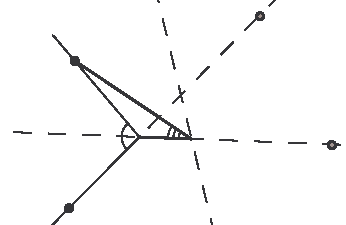
\includegraphics{../graphics/origamiTrisection.pdf}
%% \]
%% \end{con}


\newpage

\subsection*{Problems for Section~\thesection}\hrule\vspace{1ex}
\begin{enumerate}
\item What are the rules for folding and tracing constructions?
\item Use folding and tracing to bisect a given line segment. Explain the steps in
  your construction.
\item Given a line segment with a point on it, use folding and tracing to
  construct a line perpendicular to the segment that passes through
  the given point. Explain the steps in your construction.
\item Use folding and tracing to bisect a given angle. Explain the steps in your
  construction.
\item Given a line and a point not on the line, use folding and tracing to construct a line parallel
  to the given line that passes through the given point. Explain the
  steps in your construction.
\item Given a line and a point not on the line, use folding and tracing to construct a line
  perpendicular to the given line that passes through the given
  point. Explain the steps in your construction.
\item Given a circle (a center and a point on the circle) and a line,
  use folding and tracing to construct the intersection. Explain the steps in your
  construction.
\item Given a line segment, use folding and tracing to construct an equilateral
  triangle whose edge has the length of the given segment. Explain the
  steps in your construction.
\item Explain how to use folding and tracing to transfer a segment.
\item Given an angle and a point, use folding and tracing to copy the angle so
  that the new angle has  the given point as its vertex. Explain the
  steps in your construction.
\item Explain how to use folding and tracing to construct an envelope of tangents for
  a parabola.
\item Given the length of one side, use folding and tracing to construct a square. Explain the steps in your construction.
\item Given the length of one side, use folding and tracing to construct a regular hexagon. Explain the steps in
  your construction.
\item Morley's Theorem states:\index{Morley's Theorem}
If you trisect the angles of any triangle with lines, then those lines
form a new equilateral triangle inside the original triangle.\index{equilateral triangle}\index{trisecting the angle}
\[
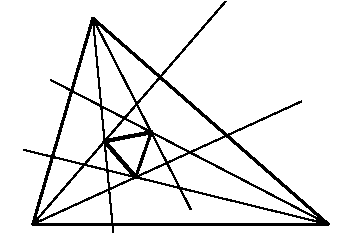
\includegraphics[scale=.5]{../graphics/morley.pdf}
\]
Give a folding and tracing construction illustrating Morley's Theorem. Explain the
steps in your construction.
\item Given a segment of length $1$, construct a triangle whose perimeter is a
  multiple of $6$. Explain the steps in your construction.
\item Given a segment of length $1$, construct a $30$-$60$-$90$ right triangle. Explain the steps in your
  construction.
\item Given a segment of length $1$, construct a triangle with a perimeter of
  $3 + \sqrt{5}$. Explain the steps in your construction.
\end{enumerate}


\newpage


\section{Anatomy of Figures}


Remember, in studying geometry we seek to discover the points that can
be obtained given a set of rules. For our purposes, the set of rules consists of the
rules for folding and tracing constructions.

\begin{ques} 
With regard to folding and tracing constructions, what is a \textit{point}?
\end{ques}
\QM

\begin{ques}
With regard to folding and tracing constructions, what is a \textit{line}?
\end{ques}
\QM


\begin{ques}
With regard to folding and tracing constructions, what is a \textit{circle}?
\end{ques}
\QM


OK, those are our basic figures: pretty easy, right? Now I'm going to
quiz you about them (I know we've already gone over this, but it is
fundamental so just smile and answer the questions):

\begin{ques} 
Place two points randomly in the plane. Do you expect to be able to
draw a single line that connects them?
\end{ques}
\QM

\begin{ques} 
Place three points randomly in the plane. Do you expect to be able to
draw a single line that connects them?
\end{ques}
\QM

\begin{ques} 
Place two different lines randomly in the plane. How many points do you expect
them to share?
\end{ques}
\QM


\begin{ques} 
Place three different lines randomly in the plane. How many points do you expect
all three lines to share?
\end{ques}
\QM


\begin{ques} 
Place three points randomly in the plane. Will you (almost!) always be
able to draw a circle containing these points? If no, why not? If yes,
how do you know?
\end{ques}
\QM


%%%%%%%%%%%%%%%%%%%%%%%%%%%%%%%%%%%%%%%%%%%%%%%%%%%%%%%%%%%%%%%
%%%%%%%%%%%%%%%%%%%%%%%%%%%%%%%%%%%%%%%%%%%%%%%%%%%%%%%%%%%%%%%
%\subsection{Parallel Lines}
%
%When working with geometry in the plane we have the following fact:
%
%\begin{quote}
%Given a line and a point there is a unique line parallel to the first
%line that passes through the given point.
%\end{quote}
%
%If you recall the Construction of a Parallel through a Point, you
%might say that this fact is self-evident. The key word in the
%statement above is \textit{unique}. This means ``one and only.''
%
%HERE HERE HERE HERE HERE HERE
%
% HOW TO DO THIS JUSTICE???
% I was thinking to use ASA and Euclid's axioms - but is that 
% the right way to go? I'm just not sure - maybe I should see 
% what they do in the Missouri books.
%%%%%%%%%%%%%%%%%%%%%%%%%%%%%%%%%%%%%%%%%%%%%%%%%%%%%%%%%%%%%%%
%%%%%%%%%%%%%%%%%%%%%%%%%%%%%%%%%%%%%%%%%%%%%%%%%%%%%%%%%%%%%%%


\subsection{Lines Related to Triangles}

Believe it or not, in mathematics we often try to study the simplest
objects as deeply as possible. After the objects listed above,
triangles are among the most basic of geometric figures, yet there is
much to know about them.  There are several lines that are commonly
associated to triangles. Here they are:
\begin{itemize}
\item Perpendicular bisectors of the sides.
\item Bisectors of the angles.
\item Altitudes of the triangle.
\item Medians of the triangle. 
\end{itemize}

The first two lines above are self-explanatory. The next two need definitions.

\begin{dfn}\index{altitude} 
An \textbf{altitude} of a triangle is a line segment originating at a
vertex of the triangle that meets the line containing the opposite
side at a right angle.
\end{dfn}


\begin{dfn}\index{median} 
A \textbf{median} of a triangle is a line segment that connects a
vertex to the midpoint of the opposite side.
\end{dfn}

\begin{ques} 
The intersection of any two lines containing the altitudes of a
triangle is called an \textbf{orthocenter}\index{orthocenter}. How
many orthocenters does a given triangle have?
\end{ques}
\QM


\begin{ques} 
The intersection of any two medians of a triangle is called a
\textbf{centroid}\index{centroid}. How many centroids does a given
triangle have?
\end{ques}
\QM


\begin{ques} What is the physical meaning of a centroid?
\end{ques}
\QM




\subsection{Circles Related to Triangles}


There are also two circles that are commonly associated to
triangles. Here they are:
\begin{itemize}
\item The circumcircle.
\item The incircle.
\end{itemize}

These aren't too bad. Check out the definitions.

\begin{dfn}\index{circumcircle}\index{circumcenter}
The \textbf{circumcircle} of a triangle is the circle that contains
all three vertices of the triangle. Its center is called the
\textbf{circumcenter} of the triangle.
\[
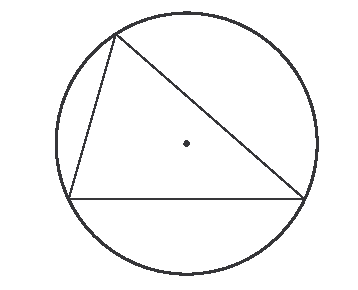
\includegraphics[width=2in]{../graphics/circumcircle.pdf}
\]
\end{dfn}

\begin{ques} Does every triangle have a circumcircle?
\end{ques}
\QM

\begin{dfn}\index{incircle}\index{incenter}
The \textbf{incircle} of a triangle is the largest circle that will
fit inside the triangle. Its center is called the \textbf{incenter} of
the triangle.
\[
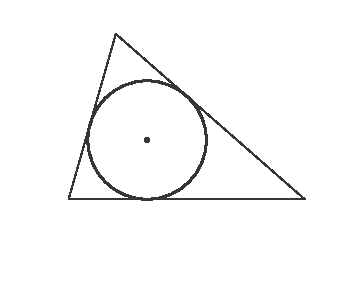
\includegraphics[width=2in]{../graphics/incircle.pdf}
\]
\end{dfn}


\begin{ques} Does every triangle have an incircle?
\end{ques}
\QM


\begin{ques} 
Are any of the lines we described related to these circles and/or
centers? Clearly articulate your thoughts.
\end{ques}
\QM


\newpage



\subsection*{Problems for Section~\thesection}\hrule\vspace{1ex}
\begin{enumerate}
\item With regard to folding and tracing constructions, what is a \textit{circle}?
  Compare and contrast this to a naive notion of a circle.
\item Place three points in the plane. Give a detailed discussion
  explaining how they may or may not be on a line.
\item Place three lines in the plane. Give a detailed discussion explaining
  how they may or may not intersect.
\item Explain how a perpendicular bisector is different from an
  altitude. Draw an example to illustrate the difference.
\item Explain how a median is different from an angle bisector.  Draw an
  example to illustrate the difference.
\item What is the name of the point that is the same distance from all
  three sides of a triangle? Explain your reasoning.
\item What is the name of the point that is the same distance from all
  three vertices of a triangle? Explain your reasoning.
\item Could the circumcenter be outside the triangle? If so, draw a
  picture and explain. If not, explain why not using pictures as
  necessary.
\item Could the orthocenter be outside the triangle? If so, draw a
  picture and explain. If not, explain why not using pictures as
  necessary.
\item Could the incenter be outside the triangle? If so, draw a
  picture and explain. If not, explain why not using pictures as
  necessary.
\item Could the centroid be outside the triangle? If so, draw a
  picture and explain. If not, explain why not using pictures as
  necessary.
\item Are there shapes that do not contain their centroid? If so, draw
  a picture and explain. If not, explain why not using pictures as
  necessary.
\item Draw an equilateral triangle. Now draw the lines containing the
  altitudes of this triangle. How many orthocenters do you have as
  intersections of lines in your drawing? Hints:
\begin{enumerate}
\item More than one.
\item How many triangles are in the picture you drew?
\end{enumerate}
\item Given a triangle, use folding and tracing to construct the circumcenter. Explain the steps
  in your construction.\index{circumcenter}
\item Given a triangle, use folding and tracing to construct the orthocenter. Explain the steps
  in your construction.\index{orthocenter}
\item Given a triangle, use folding and tracing to construct the incenter. Explain the steps in
  your construction.\index{incenter}
\item Given a triangle, use folding and tracing to construct the centroid. Explain the steps in
  your construction.\index{centroid}
\item Given a triangle, use folding and tracing to construct the incircle. Explain the steps in
  your construction.\index{incircle}
\item Given a triangle, use folding and tracing to construct the circumcircle. Explain the steps
  in your construction.\index{circumcircle}
\item Where is the circumcenter of a right triangle? Explain your
  reasoning.
\item Where is the orthocenter of a right triangle? Explain your
  reasoning.
\item Can you draw a triangle where the circumcenter, orthocenter,
  incenter, and centroid are all the same point?  If so, draw a
  picture and explain. If not, explain why not using pictures as
  necessary.
\item True or False: Explain your conclusions.
\begin{enumerate}
\item An altitude of a triangle is always perpendicular to a line
  containing some side of the triangle.
\item An altitude of a triangle always bisects some side of the
  triangle.
\item The incenter is always inside the triangle.
\item The circumcenter can be outside the triangle.
\item The orthocenter is always inside the triangle.
\item The centroid is always inside the incircle.
\end{enumerate}
\item Given 3 distinct points not all in a line, construct a circle
  that passes through all three points. Explain the steps in your
  construction.
\item The following picture shows a triangle that has been folded
  along the dotted lines:
\[
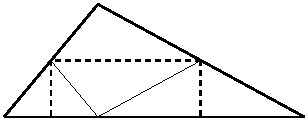
\includegraphics{../graphics/origamiPBPTri.pdf}
\]
Explain how the picture ``proves'' the following statements:
\begin{enumerate}
\item The interior angles of a triangle sum to $180^\circ$. 
\item The area of a triangle is given by $bh/2$ for $b$ the length of the base and $h$ the height of the triangle. 
\end{enumerate}
\item Use folding and tracing to construct a triangle given the length of one
  side, the length of the the median to that side, and the length of
  the altitude of the opposite angle. Explain the steps in your
  construction.
\item Use folding and tracing to construct a triangle given one angle, the length
  of an adjacent side and the altitude to that side. Explain the steps
  in your construction.
\item Use folding and tracing to construct a triangle given one angle and the
  altitudes to the other two angles. Explain the steps in your
  construction.
\item Use folding and tracing to construct a triangle given two sides and the
  altitude to the third side. Explain the steps in your construction.
\end{enumerate}

\newpage


\section{Similar Triangles}


In geometry, we may have several different segments all with the same
length. We don't want to say that the segments are \textit{equal}
because that would mean that they are \textit{exactly} the
same---position included. Hence we need a new concept:

\begin{dfn}\index{congruent!segments}
When different segments have the same length, we say they are
\textbf{congruent segments}. 
\end{dfn}

\begin{dfn}\index{congruent!angles}
In a similar fashion, if there is an isometry that maps one angle to another angle, then we say they are \textbf{congruent angles}.
\end{dfn}

Putting these together, we have the definition for triangles:

\begin{dfn}\index{congruent!triangles} 
Two triangles are said to be \textbf{congruent triangles} if there is
an isometry that maps one triangle to the other triangle.
\end{dfn}


After working with triangles for short time, one quickly sees that the
notion of congruence is not the only ``equivalence'' one wants to
make between triangles. In particular, we want the notion of
\textit{similarity.} \index{similar triangles}

One day when aloof old Professor Rufus was trying to explain similar
triangles to his class, he merely wrote
\[
\tri ABC \sim \tri A'B'C' \qquad\Leftrightarrow \qquad\begin{array}{l}
\angle A \simeq \angle A'\\
\angle B \simeq \angle B' \\
\angle C \simeq \angle C'
\end{array}
\]
and walked out of the room.

\begin{ques} 
Can you give three much needed examples of similar triangles? 
\end{ques}
\QM

\begin{ques} 
Devise a way to use folding and tracing constructions to help explore this notion
of similar triangles.
\end{ques}
\QM

Another day when aloof old Professor Rufus was trying to explain
similar triangles to his class, he merely wrote
\[
\tri ABC \sim \tri A'B'C' \qquad\Leftrightarrow \qquad
\begin{array}{l}
AB = k\cdot A'B'\\
BC = k\cdot B'C' \\
CA = k\cdot C'A'
\end{array}
\]
and walked out of the room.

\begin{ques} 
Can you give three much needed examples of similar triangles? 
\end{ques}
\QM

\begin{ques} 
Devise a way to use folding and tracing constructions to help explore this notion
of similar triangles.
\end{ques}
\QM



\begin{ques} 
What's going on in aloof old Professor Rufus' head\footnote{I realize that
this is a dangerous question!}---why are his explanations so different?
\end{ques}
\QM

In fact, the two definitions of similar triangles given
above are \textbf{equivalent}.


\begin{dfn}\index{similar triangles} 
Two triangles $\tri ABC$ and $\tri A'B'C'$ are said to be
\textbf{similar} if either equivalent condition holds:
\[
\begin{array}{l}
\angle A \simeq \angle A'\\
\angle B \simeq \angle B' \\
\angle C \simeq \angle C'
\end{array}
\qquad\text{or}\qquad
\begin{array}{l}
AB = k\cdot A'B'\\
BC = k\cdot B'C' \\
CA = k\cdot C'A'
\end{array}
\]
\end{dfn}

Let's see if we can put similar triangles to work. Here is an old
carpenter's trick. Suppose you have two parallel lines.  
\[
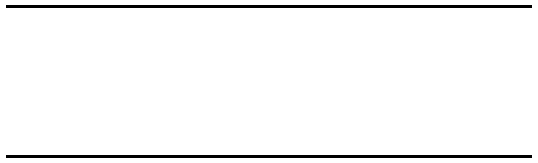
\includegraphics{../graphics/twoLinesCarp.pdf}
\]
If you want to make two more lines that divide the space into three
equal regions, you can place a ruler diagonally across the parallel
lines, and then mark off one-third of the diagonal distance. 
\[
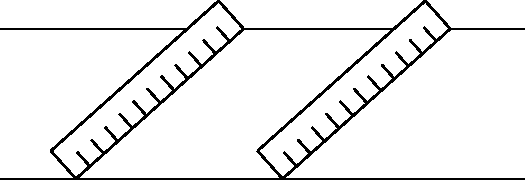
\includegraphics{../graphics/twoLinesCarpRulers.pdf}
\]
From this you get your three regions.
\[
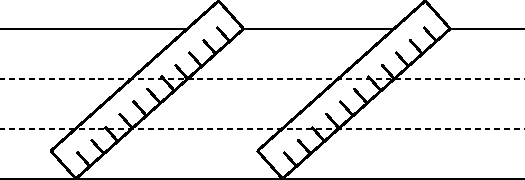
\includegraphics{../graphics/twoLinesCarpRulersLines.pdf}
\]
\begin{ques}
Can you explain why this works using similar triangles?
\end{ques}
\QM

Now for a more challenging situation.  Suppose we have an equilateral
triangle of side length 2. Use similar triangles and the Pythagorean
Theorem to find the length of the segment $a$ (the segment that goes
from the \textbf{center} of the triangle to a side at a right angle)
in the picture below.
\[
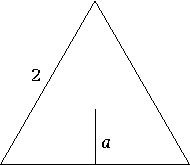
\includegraphics{../graphics/triangleSegment.pdf}
\]
\begin{ques}
How do you do this?
\end{ques}
\QM

\newpage


\subsection*{Problems for Section~\thesection}\hrule\vspace{1ex}
\begin{enumerate}
\item Compare and contrast the ideas of \textit{equal triangles},
  \textit{congruent triangles}, and \textit{similar triangles}.
\item Explain why all equilateral triangles are similar to each other.
\item Explain why all isosceles right triangles are similar to each other. 
\item Explain why when given a right triangle, the altitude of the
  right angle divides the triangle into two smaller triangles each
  similar to the original right triangle.
\item The following sets contain lengths of sides of similar
  triangles. Solve for all unknowns---give all solutions. In each case,
  explain your reasoning.
\begin{enumerate}
\item $\{3,4,5\}$, $\{6,8,x\}$
\item $\{3,3,5\}$, $\{9,9,x\}$
\item $\{5,5,x\}$, $\{10,4,y\}$
\item $\{5,5,x\}$, $\{10,8,y\}$
\item $\{3,4,x\}$, $\{4,5,y\}$ 
\end{enumerate}
\item A \textit{Pythagorean Triple}\index{Pythagorean Triple} is a set
  of three positive integers $\{a,b,c\}$ such that $a^2 + b^2 =
  c^2$. Write down an infinite list of Pythagorean Triples. Explain
  your reasoning and justify all claims.
\item Here is a right triangle, note that it is \textbf{not} drawn to
  scale:
\[
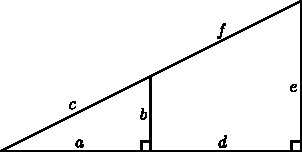
\includegraphics{../graphics/origamiSimQ.pdf}
\]
Solve for all unknowns in each of the following cases.
\begin{enumerate}
\item $a = 3$, $b = ?$, $c = ?$, $d = 12$, $e = 5$, $f = ?$
\item $a = ?$, $b = 3$, $c = ?$, $d =8$, $e = 13$, $f = ?$
\item $a = 7$, $b = 4$, $c = ?$, $d =?$, $e = 11$, $f = ?$
\item $a = 5$, $b = 2$, $c = ?$, $d =6$, $e = ?$, $f = ?$
\end{enumerate}
In each case, explain your reasoning.

\item Suppose you have two similar triangles. What can you say about
  the area of one in terms of the area of the other? Be specific and
  explain your reasoning.

\item During a solar eclipse we see that the apparent diameter of the
  Sun and Moon are nearly equal. If the Moon is around $24000$ miles
  from Earth, the Moon's diameter is about $2000$ miles, and the Sun's
  diameter is about $865000$ miles, how far is the Sun from the Earth?
\begin{enumerate}
\item Draw a relevant (and helpful) picture showing the important
  points of this problem.
\item Solve this problem, and be sure to explain your reasoning.
\end{enumerate}


\item When jets fly above $8000$ meters in the air they form a vapor
  trail. Cruising altitude for a commercial airliner is around $10000$
  meters. One day I reached my arm into the sky and measured the
  length of the vapor trail with my hand---my hand could just span the
  entire trail. If my hand spans $9$ inches and my arm extends $25$
  inches from my eye, how long is the vapor trail? Explain your
  reasoning.
\begin{enumerate}
\item Draw a relevant (and helpful) picture showing the important
  points of this problem.
\item Solve this problem, and be sure to explain your reasoning.
\end{enumerate}

\item David proudly owns a 42 inch (measured diagonally) flat screen
  TV. Michael proudly owns a 13 inch (measured diagonally) flat screen
  TV. David sits comfortably with his dog Fritz at a distance of 10
  feet. How far must Michael stand from his TV to have the ``same''
  viewing experience?  Explain your reasoning.
\begin{enumerate}
\item Draw a relevant (and helpful) picture showing the important
  points of this problem.
\item Solve this problem, and be sure to explain your reasoning.
\end{enumerate}

\item You love IMAX movies. While the typical IMAX screen is 72 feet
  by 53 feet, your TV only has a 32 inch screen---it has a 32 inch
  diagonal. How close do you have to sit to your screen to simulate
  the IMAX format? Explain your reasoning.
\begin{enumerate}
\item Draw a relevant (and helpful) picture showing the important
  points of this problem.
\item Solve this problem, and be sure to explain your reasoning.
\end{enumerate}

\item David proudly owns a 42 inch (measured diagonally) flat screen
  TV. Michael proudly owns a 13 inch (measured diagonally) flat screen
  TV. Michael stands and watches his TV at a distance of 2 feet. David
  sits comfortably with his dog Fritz at a distance of 10 feet. Whose
  TV appears bigger to the respective viewer? Explain your reasoning.
\begin{enumerate}
\item Draw a relevant (and helpful) picture showing the important
  points of this problem.
\item Solve this problem, and be sure to explain your reasoning.
\end{enumerate}

\item Here is a personal problem: Suppose you are out somewhere and
  you see that when you stretch out your arm, the length of your thumb
  is the same apparent size as a distant object. How far away is the
  object if you know the object is:
\begin{enumerate}
\item 6' long (as tall as a person).
\item 16' long (as long as a car).
\item 40' long (as long as a school bus).
\item 220' long (as long as a large passenger airplane).
\item 340' long (as long as an aircraft carrier).
\end{enumerate}
Explain your reasoning.

\item I was walking down Woody Hayes Drive, standing in front of
  St.\ John Arena when a car pulled up and the driver asked, ``Where
  is Ohio Stadium?'' At this point I was a bit perplexed, but
  nevertheless I answered, ``Do you see the enormous concrete building
  on the other side of the street that looks like the Roman Colosseum?
  That's it.''
 
The person in the car then asked, ``Where are the Twin-Towers then?''
Looking up, I realized that the towers were in fact just covered by the
top of Ohio Stadium. I told the driver to just drive around the
stadium until they found two enormous identical towers---that would be
them. They thanked me and I suppose they met their destiny.

I am about 2 meters tall, I was standing about 100 meters from the
Ohio Stadium, and Ohio Stadium is about 40 meters tall. If the Towers
are around 500 meters from the rotunda (the front entrance of the
stadium), how tall could they be and still be obscured by the stadium?
Explain your reasoning---for the record, the towers are about 80
meters tall.


\item Consider the following combinations of S's and A's. Which of
  them produce a \textit{Congruence Theorem}? Which of them produce a
  \textit{Similarity Theorem}? Explain your reasoning.
\[
\text{SSS},\quad \text{SSA},\quad \text{SAS},\quad 
\text{SAA},\quad \text{ASA},\quad \text{AAA} 
\]


\item Explain how the following picture ``proves'' the Pythagorean Theorem.
\[
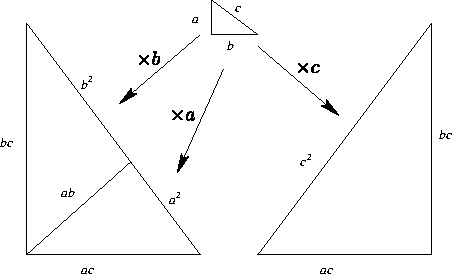
\includegraphics{../graphics/pbpdilation.pdf}
\]


\end{enumerate}

%\item \label{P:CP} Given a circle centered at point $O$, we'll call
%  two points $P$ and $P'$ a \textit{connected pair} if:
%\begin{enumerate}
%\item $O$, $P$, and $P'$ all lie on a line.
%\item $OP = \dfrac{1}{OP'}$.
%\end{enumerate}
%For example, if the radius of the circle was $12$ and $P$ was $6$
%units from $O$, then $P'$ would be $18$ units from $O$. Give some
%other examples of connected pairs.
%\item If $P$ and $P'$ are a connected pair (see Problem~\ref{P:CP})
%  and $P$ is on the circle, what can you say about $P'$? Explain your
%  reasoning.
%\item Consider the following diagram where $P$ and $P'$ are connected
%  pairs (see Problem~\ref{P:CP}):
%\[
%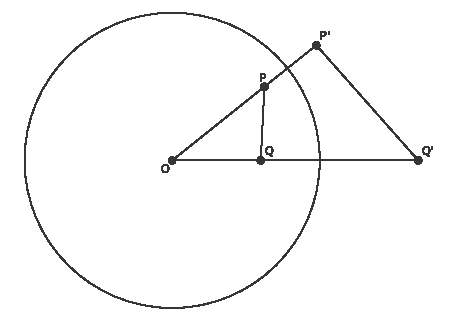
\includegraphics{../graphics/origamiConnected.pdf}
%\]
%What is the distance $P'Q'$? Hint: Try to use the SAS-Similarity
%Theorem, to do this you'll have to find some sides with common ratios!







